\documentclass[12pt]{article}
\usepackage[latin1,utf8]{inputenc}
\usepackage[brazil]{babel}
\usepackage{setspace}
\usepackage{boxedminipage}
\usepackage{latexsym}
\usepackage{multirow}
\usepackage[pdftex]{graphicx}
\usepackage{float}
\usepackage{url}
\usepackage{xcolor,listings}
\usepackage{amsmath,mathrsfs}
\usepackage{biblatex}
\usepackage[portuguese, ruled, linesnumbered]{algorithm2e}
\usepackage{enumitem}
\addbibresource{references.bib}

%\setlength{\parskip}{0.1cm}
\setlength{\paperheight}{29.7cm}
\setlength{\textheight}{23.0cm}
\setlength{\textwidth}{16.5cm}
\setlength{\oddsidemargin}{0.0cm}
\setlength{\topmargin}{-1.0cm}
\pagestyle{empty}

% Custom colors
\usepackage{color}
\definecolor{deepblue}{rgb}{0,0,0.5}
\definecolor{deepred}{rgb}{0.6,0,0}
\definecolor{deepgreen}{rgb}{0,0.5,0}

\begin{document}

\lstset{language=python,
    keywordstyle=\color{deepblue}\bfseries,
    commentstyle=\color{deepgreen},
    stringstyle=\ttfamily\color{deepred!50!brown},
    breaklines=true,
    showstringspaces=false}
\lstset{literate=%
   *{0}{{{\color{red!20!violet}0}}}1
    {1}{{{\color{red!20!violet}1}}}1
    {2}{{{\color{red!20!violet}2}}}1
    {3}{{{\color{red!20!violet}3}}}1
    {4}{{{\color{red!20!violet}4}}}1
    {5}{{{\color{red!20!violet}5}}}1
    {6}{{{\color{red!20!violet}6}}}1
    {7}{{{\color{red!20!violet}7}}}1
    {8}{{{\color{red!20!violet}8}}}1
    {9}{{{\color{red!20!violet}9}}}1
}

\begin{center}
{\sf {\large Visão e Processamento de Imagens - Avaliação única -
    Parte II}}

\textbf{Preste atenção para as regras da prova}
\end{center}
1- O fonte latex (.tex) da prova será disponibilizado para facilitar
que você não tenha que copiar o enunciado das questões. Todas as questões
devem ser respondidas no mesmo arquivo.

\noindent 2- A prova é \textbf{individual}.  É permitido a consulta a
livros, apontamentos ou Internet, desde que devidamente referenciada.
Não é permitida a consulta a colegas, amigos, família, cachorro,
papagaio e etc. 

\noindent 3- A prova deve ser entregue diretamente no Paca, assim como
todos os códigos e imagens devem ser entregues no mesmo arquivo
comprimido.  \textbf{Duração da prova: 14 dias}.  

\noindent 4- Cada questão vale 20 pontos (pois são apenas 3 questões)
para a graduação e 15 pontos para a pós-graduação (pois são 4 questões). 
\bigskip

\begin{itemize}
\item[{\bf Q1.}] Para fazer esta questão, leia primeiro o artigo abaixo:
\begin{itemize}
\item \url{http://www.eecs.berkeley.edu/Pubs/TechRpts/2015/EECS-2015-85.pdf}
\end{itemize} 
\begin{itemize}
\item Faça um resumo do artigo de acordo com as indicações que deixei no paca (artigos sobre como fazer um resumo).

\begin{enumerate}
  \item Summary \(40\% : 2.5 pages\)
    \begin{enumerate}[label*=\arabic*.]
      \item Motivation \(8\%\)
      \item Contribution \(8\%\)
      \item Methodology \(16\%\)
      \item Conclusion \(8\%\)
    \end{enumerate}
  \item Critique \(30\% : 1.5 pages\)
    \begin{enumerate}[label*=\arabic*.]
      \item Title of 1st Critique \(15\%\)
       \item Title of 2nd Critique \(15\%\)
       \item Optional: Title of 3rd Critique
    \end{enumerate}
  \item Synthesis \(30\% : 1 page\)
    \begin{enumerate}[label*=\arabic*.]
      \item Title of 1st Idea \(30\%\)
      \item Optional: Title of 2nd Idea
    \end{enumerate}
\end{enumerate}
1. What is the research problem the paper attempts to address?
O artigo contextualiza o cenário atual no que diz respeito à manipulação de imagens 
por ferramentas de edição, ressaltando a ampla gama de técnicas que essas ferramentas
possuem e que permitem aos seus usuários a manipulação de imagens que implica em uma análise
detalhista por um profissional especializado para descobrir algum tipo de fraude.

What is the motivation of the research work?
Não obstante, a motivação principal do trabalho proposto é de criar uma ferramenta capaz de
avaliar uma dada imagem, de forma que qualquer pessoa comum possa identificar potenciais fraudes,
sem a necessidade de auxílio de um analista forense, por exemplo.
Podemos destacar, ainda, o fato de que pessoas podem coletar evidencias de crimes ou 
eventos quaisquer de uma forma trivial considerando a difusão de dispositivos móveis 
equipados com cameras de boa qualidade.

Is there a crisis in the research field that the paper attempts to resolve?
Podemos afirmar que ainda não há crise na área pesquisada, porém, tendencias de mercado
norteiam para que processos historicamente feitos sob arquivos impressos e com a presença
dos envolvidos, sejam totalmente realizados por plataformas online, o que pode, futuramente,
causar grandes transtornos às empresas e ao estado de um modo geral pelo risco de desvio de conduta
e possibilidades de fraudes em processos sigilosos, de grande valor agregado, avaliações contratuais, etc.
Não é demasiado lembrar que processos judiciais já são interpretados com ajuda de imagens digitais, o que 
nos remete a necessidade de garantir a autenticidade das mesmas, assim como também no jornalismo, 
cuja integridade pode ser colocada em xeque em casos de adulteração de fotos em quaisquer publicações.

Is the research work attempting to overcome the weaknesses of existing approaches?
Is an existing research paradigm challenged? In short, what is the niche of the paper?

2. What are the claimed contributions of the paper? What is new in this paper?
A new question is asked?
A new understanding of the research problem?
A new methodology for solving problems?
A new algorithm?
A new breed of software tools or systems?
A new experimental method?
A new proof technique?
A new formalism or notation?
A new evidence to substantiate or disprove a previously published claim?
A new research area?
In short, what is innovative about this paper?

3. How do the authors substantiate their claims?
What is the methodology adopted to substantiate the claims?
What is the argument of the paper? What are the major theorems?
What experiments are conducted?
Data analyses?
Simulations?
Benchmarks?
User studies?
Case studies?
Examples?
In short, what makes the claims scientific (as opposed to being mere opinions1)?

4. What are the conclusions?
What have we learned from the paper?
Shall the standard practice of the field be changed as a result of the new findings?
Is the result generalizable?
Can the result be applied to other areas of the field?
What are the open problems?
In short, what are the lessons one can learn from the paper?


\item Implemente o método ELA (Error Level Analysis) em Python (apresente o 
\textbf{algoritmo} na prova e anexe o código em Python no arquivo zip).

Abaixo o algoritmo que foi implementado onde utilizei o pacote $pillow$ do python para as operações na imagem.
O código completo está em \textbf{source/ela.py}.

%Código
\begin{algorithm}[H]
    \SetKwData{Img}{ImagemOriginal}
    \SetKwData{ResavedImg}{ImagemComprimida}
    \SetKwData{ElaImg}{ImagemELA}
    \SetKwData{ImgPath}{Caminho\quad da\quad imagem}
    \SetKwData{ResavedPath}{Caminho\quad da\quad imagem comprimida}
    \SetKwFunction{abrirImagem}{abrirImagem}
    \SetKwFunction{salvarImagem}{salvarImagem}
    
    \SetAlgoLined
    \Entrada{Caminho\quad da\quad imagem, escala}
    \Saida{Imagem com ELA calculado}
    \BlankLine
    \Img $\leftarrow$ \abrirImagem{\ImgPath}\\
    \Se{\Img não é JPEG}{\Retorna{Nulo}}
    \BlankLine
    \salvarImagem{\ResavedPath, JPEG, qualidade}\\
    \ResavedImg $\leftarrow$ \abrirImagem{\ResavedPath}\\
    \BlankLine
    \Para{$x\leftarrow 0$ \Ate $largura\quad \Img$}{
        \Para{$y\leftarrow 0$ \Ate $altura\quad \Img$}{
            $pixel\_img\_original = \Img[x,y]$\\
            $pixel\_img\_comprimida = \ResavedImg[x,y]$\\
            $R = abs(pixel\_img\_original[0] - pixel\_img\_comprimida[0]) * escala$\\
            $G = abs(pixel\_img\_original[1] - pixel\_img\_comprimida[1]) * escala$\\
            $B = abs(pixel\_img\_original[2] - pixel\_img\_comprimida[2]) * escala$\\
            $\ElaImg[x,y] = [R, G, B]$
        }
    }
    \BlankLine
    \Retorna{\ElaImg}
    \label{alg1}
    \caption{\textsc{Error Level Analysis}}
\end{algorithm}

\item Teste seu algoritmo com as imagens que deixei no paca para este exercício. 
Quantas imagens seriam consideradas modificadas por esse método? Comente o resultado,
comparando com a sua intuição.

Uma vez submetida a imagem ao \textit{Error Level Analysis}, pode-se perceber pelo resultado que 
a região manipulada terá um nível de erro diferente das regiões não manipuladas. Logo, 
o nível de erro irá expor a região manipulada rotulando as regiões com maior alteração após
a imagem ser salva com um nível de qualidade inferior \cite{krawetz}.

Na Figura 1b, podemos ver o resultado do ELA na imagem dada. As regiões com maior chance de ter
alterações são as que apresentam os pixels com maior brilho, uma vez que a alteração da imagem 
causa instabilidade nestas áreas.
\begin{figure}[htb]
\centering
\begin{minipage}[b]{0.45\textwidth}
	\centering
        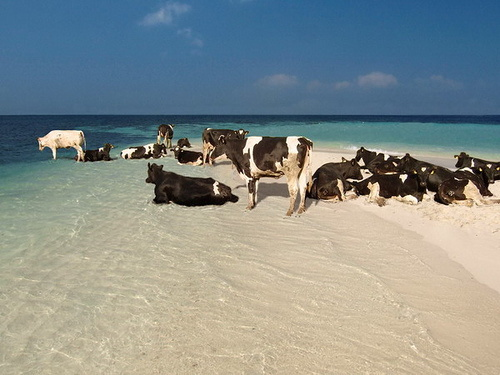
\includegraphics[scale=0.3]{Q3Images/cows_on_beach.jpg} 
	\centerline{\label{fig1a} \small (1a) Imagem original}
\end{minipage}
\begin{minipage}[b]{0.45\textwidth}
	\centering
        
\includegraphics[scale=0.3]{Q3Images/cows_on_beach_ela.png} 
	\centerline{\label{fig1b} \small (1b) Imagem com o resultado do ELA}
\end{minipage}
\end{figure}

Os resultados foram avaliados de acordo com o brilho das bordas que devem ser semelhantes no resultado 
da aplicação do ELA na imagem. Além disso, regiões de cores e texturas semelhantes na imagem
original, independentemente da cor, também devem ter cores aproximadamente similares no ELA \cite{berkeleywebsite}.

Isto posto, considerei que um total de 23 \{2000\_snowballcat.jpg, blacklion01.jpg, cows\_on\_beach.jpg, daliatom.jpg,
frozenvenice.jpg, glass\_butterfly.jpg, houseboat01.jpg, jumping\_giraffe.jpg, kissing.jpg, leap.jpg, magic\_tap.jpg,
manitoba\_security.jpg, moonmelon01.jpg, nikolatesla.jpg, rocket\_bike.jpg, sharkswim.jpg, skiing\_egypt.jpg, spacechair.jpg,
tattooguy01.jpg, tennis.jpg, tentacle\_bldg.jpg, vuitton.jpg, wienerplane.jpg\} imagens foram alteradas de acordo 
com o método e avaliação a posteriori.
\end{itemize}
%
%
%
\item[{\bf Q2.}] Esta questão refere-se à transformada de Fourier.
\begin{itemize}
\item Encontre a transformada de Fourier da função:
\begin{eqnarray*}
f(x) = \left\{ \begin{array}{rl} 
 7 &\mbox{ if $-5 < x < 5$} \\
 0 &\mbox{ caso contrário}
       \end{array} \right.
\end{eqnarray*}

Por definição, temos que a transformada de Fourier de um pulso
retangular de largura $D$ e altura $A$ tem a forma dada por:

\begin{eqnarray*}
    F(\omega) = ADsinc\bigg(\frac{\omega D}{2}\bigg)  = AD\frac{sin(\frac{\omega D}{2})}{\frac{\omega D}{2}}
\end{eqnarray*}

A função $f(x)$ pode ser representada graficamente como:
\begin{figure}[htb]
\centering   
\begin{minipage}[b]{0.45\textwidth}
	\centering
        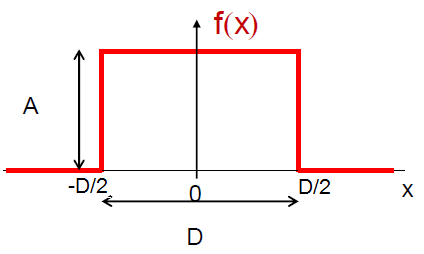
\includegraphics[scale=0.45]{Q3Images/pulse_function.png} 
\end{minipage}
\end{figure}

Onde:
\begin{eqnarray*}
f(x) = \left\{ \begin{array}{rl} 
 A, &\mbox{ $x \in  [\frac{-D}{2}, \frac{D}{2}]$} \\
 0, &\mbox{ $x \notin [\frac{-D}{2}, \frac{D}{2}]$}
       \end{array} \right.
\end{eqnarray*}

Logo, temos que A = 7 e D = 10 e, portanto, a transformada de Fourier da função $f(x)$ é:
\begin{align*}
    F(\omega) &= AD\frac{sin(\frac{\omega D}{2})}{\frac{\omega D}{2}} \\
              &= 7*10\frac{sin(\frac{\omega 10}{2})}{\frac{\omega 10}{2}} \\
              &= 70\frac{sin(\frac{\omega 10}{2})}{\frac{\omega 10}{2}} \\
              &= 70\frac{sin(5\omega)}{5\omega}
\end{align*}

%%%
\item Encontre a transformada de Fourier da função $ g(x) = f(x)\cos
   \omega_0 x$, sabendo que a transformada de Fourier de $f(x)$ é dada
   por $F(\omega)$

Tomando a propriedade da modulação:
\begin{align*}
    \mathcal{F}[x(t)cos(\omega_0t)] = \frac{1}{2}[F(\omega + \omega_0) + F(\omega - \omega_0)]
\end{align*}
Temos que a transformada de Fourier da função $g(x)$ é:
\begin{align*}
    G(\omega) = \frac{1}{2}F(\omega + \omega_0) + \frac{1}{2}F(\omega - \omega_0)
\end{align*}

%%%
\item Ache a inversa da transformada de Fourier de $G(\omega) =
  20\frac{\sin 5\omega}{5\omega}e^{-3\omega i}$

Por ora, ignorando a exponencial complexa de $G(\omega)$, podemos obter os valores de $A$ e $D$:
\begin{align*}
    20\frac{sin(5\omega)}{5\omega} = AD\frac{sin(\frac{\omega D}{2})}{\frac{\omega D}{2}} \\
    \\ 5\omega = \frac{\omega D}{2} \\
    10\omega = \omega D \\
    D = \frac{10\omega}{\omega} = 10 \\
    \\ AD = 20 \\
    A10 = 20 \\
    A = 2
\end{align*}

Como vimos no primeiro item do exercício 2, sabemos que:
\begin{align*}
f(x) = A . rect(x) = \left\{ \begin{array}{rl}
 A, &\mbox{ $x \in  [\frac{-D}{2}, \frac{D}{2}]$} \\
 0, &\mbox{ $x \notin [\frac{-D}{2}, \frac{D}{2}]$}
       \end{array} \right.
\\ A . rect\bigg(\frac{x}{D}\bigg) \xrightarrow{\mathscr{F}} ADsinc \bigg(\frac{\omega D}{2}\bigg)
\end{align*}

O que nos dá a forma do pulso retangular:
\begin{align*}
f(x) = 2 . rect\bigg(\frac{x}{10}\bigg) = \left\{ \begin{array}{rl} 
 2, &\mbox{ $x \in  [-5, 5]$} \\
 0, &\mbox{ $x \notin [-5, 5]$}
       \end{array} \right.
\end{align*}

\begin{figure}[htb]
\centering   
\begin{minipage}[b]{0.45\textwidth}
	\centering
        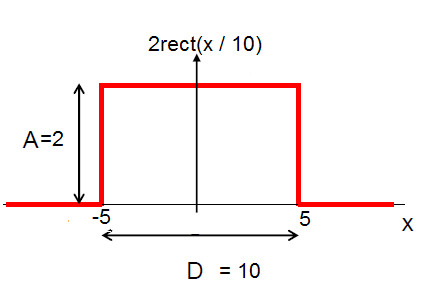
\includegraphics[scale=0.45]{Q3Images/pulse_function_2.png} 
\end{minipage}
\end{figure}

Considerando agora a exponencial complexa, sabemos que ela representa um deslocamento no tempo,
que é $3$ neste caso e, portanto:
\begin{align*}
    2 . rect\bigg(\frac{x-3}{10}\bigg) \xrightarrow{\mathscr{F}} 20\frac{\sin 5\omega}{5\omega}e^{-3\omega i} \\
    g(x) = 2 . rect\bigg(\frac{x-3}{10}\bigg) = \left\{ \begin{array}{rl} 
     2, &\mbox{ $-2 < x < 8$} \\
     0, &\mbox{ caso contrário}
           \end{array} \right.
\end{align*}
\begin{figure}[htb]
\centering   
\begin{minipage}[b]{0.45\textwidth}
	\centering
        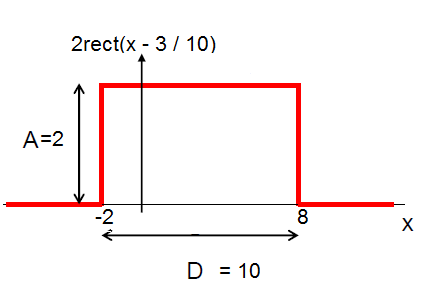
\includegraphics[scale=0.45]{Q3Images/pulse_function_3.png} 
\end{minipage}
\end{figure}


%%%
\item Calcule a DFT do sinal $f = \{1,3,5,3,1\}$

A DFT é dada por:
\begin{align*}
    F(k) = \sum\limits_{n=0}^{N-1} f(n) e^{-jk\frac{2\pi}{N}n}
\end{align*}

Para realizar os cálculos devemos utilizar a identidade de Euler:
\begin{align*}
    e^{-j \pi} = \cos \pi - j\sin\pi
\end{align*}
Devemos utilizar a seguinte equação para calcular a DFT do sinal dado por $f(x)$:
\begin{align*}
    X[k] = \sum\limits_{n=0}^{N-1} x[n] e^{-jk\frac{2\pi}{N}n},\qquad para\quad k=0,1,2,...,N-1
\end{align*}
Temos que N=5, logo:
\begin{align*}
    &X[0] = (1e^0 + 3e^0 + 5e^0 + 3e^0 + 1e^0) &\\
    &X[1] = (1e^0 + 3e^{-j1\frac{2\pi}{5}1} + 5e^{-j1\frac{2\pi}{5}2} + 3e^{-j1\frac{2\pi}{5}3} + 1e^{-j1\frac{2\pi}{5}4)} &\\
    &X[2] = (1e^0 + 3e^{-j2\frac{2\pi}{5}1} + 5e^{-j2\frac{2\pi}{5}2} + 3e^{-j2\frac{2\pi}{5}3} + 1e^{-j2\frac{2\pi}{5}4)} &\\
    &X[3] = (1e^0 + 3e^{-j3\frac{2\pi}{5}1} + 5e^{-j3\frac{2\pi}{5}2} + 3e^{-j3\frac{2\pi}{5}3} + 1e^{-j3\frac{2\pi}{5}4)} &\\
    &X[4] = (1e^0 + 3e^{-j4\frac{2\pi}{5}1} + 5e^{-j4\frac{2\pi}{5}2} + 3e^{-j4\frac{2\pi}{5}3} + 1e^{-j4\frac{2\pi}{5}4)} &\\
    &X[0] = (1 + 3 + 5 + 3 + 1) &\\
    &X[1] = (1 + 3e^{-j\frac{2\pi}{5}} + 5e^{-j\frac{4\pi}{5}}  + 3e^{-j\frac{6\pi}{5}}  + 1e^{-j\frac{8\pi}{5})} &\\
    &X[2] = (1 + 3e^{-j\frac{4\pi}{5}} + 5e^{-j\frac{6\pi}{5}}  + 3e^{-j\frac{12\pi}{5}} + 1e^{-j\frac{16\pi}{5})} &\\
    &X[3] = (1 + 3e^{-j\frac{6\pi}{5}} + 5e^{-j\frac{12\pi}{5}} + 3e^{-j\frac{18\pi}{5}} + 1e^{-j\frac{24\pi}{5})} &\\
    &X[4] = (1 + 3e^{-j\frac{8\pi}{5}} + 5e^{-j\frac{16\pi}{5}} + 3e^{-j\frac{24\pi}{5}} + 1e^{-j\frac{32\pi}{5})}&
\end{align*}
Calculando cada componente com a relação de Euler e substituindo os resultados na equação acima:
\begin{align*}
    &e^{-j\frac{2\pi}{5}} = cos(\frac{2\pi}{5}) - jsen(\frac{2\pi}{5}) = 0,30902  - 0,95106j &\\
    &e^{-j\frac{4\pi}{5}} = cos(\frac{4\pi}{5}) - jsen(\frac{4\pi}{5}) = -0,80902 - 0,58779j &\\
    &e^{-j\frac{6\pi}{5}} = cos(\frac{6\pi}{5}) - jsen(\frac{6\pi}{5}) = -0,80902 + 0,58779j &\\
    &e^{-j\frac{8\pi}{5}} = cos(\frac{8\pi}{5}) - jsen(\frac{8\pi}{5}) = 0,30902  - 0,95106j &\\
    &e^{-j\frac{12\pi}{5}} = cos(\frac{12\pi}{5}) - jsen(\frac{12\pi}{5}) = 0,30902	-0,95106j &\\
    &e^{-j\frac{16\pi}{5}} = cos(\frac{16\pi}{5}) - jsen(\frac{16\pi}{5}) = -0,80902 + 0,58779j &\\
    &e^{-j\frac{18\pi}{5}} = cos(\frac{18\pi}{5}) - jsen(\frac{18\pi}{5}) = 0,30902 + 0,95106j &\\
    &e^{-j\frac{24\pi}{5}} = cos(\frac{24\pi}{5}) - jsen(\frac{24\pi}{5}) = -0,80902 - 0,58779j &\\
    &e^{-j\frac{32\pi}{5}} = cos(\frac{32\pi}{5}) - jsen(\frac{32\pi}{5}) = 0,30902	- 0,95106j&
\end{align*}
Temos então que o resultado da DFT é:
\begin{multline*}
    X[f] = 13, -4.236067-3.077683j, 0.236067+0.726542j, \\
           0.236067-0.726542j, -4.236067+3.077683j
\end{multline*}

\end{itemize}
%
%
%
\item[{\bf Q3.}] 
\begin{itemize}
\item Calcule (apresente os cálculos) dos descritores de Fourier das
  figuras 3a e 3b. Lembre-se que os pontos da
  borda do quadrado serão representados por pontos no plano de
  Argand-Gauss. Isto é, cada ponto no plano passa a ser um número
  complexo e a borda passa a ser um vetor de pontos complexos, como
  num sinal, mas com valores complexos.

\textbf{TODO}

\item Para confirmar que seus cálculos estão corretos, implemente um
  programa em Python que receba como entrada um vetor de números
  complexos (que são as coordenadas das bordas) e retorne os
  descritores de Fourier do vetor de entrada. Você pode usar as
  funções fornecidas pela biblioteca NUMPY para facilitar a
  programação.
  
\textbf{TODO}

\item Para reconstruir a curva, faça uma função que receba um vetor
  com os descritores de Fourier, um número $N$ de descritores a serem
  usados e grafique os pontos num plano cartesiano (para fazer a mesma 
figura que fizemos nos slides das aulas 15 e 16.

\textbf{TODO}

\end{itemize}
\begin{figure}[htb]
\centering
\begin{minipage}[b]{0.45\textwidth}
	\centering
        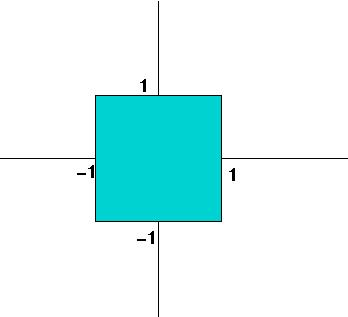
\includegraphics[scale=0.2]{Q3Images/square1.jpg} 
	\centerline{\label{fig3a} \small (3a) Quadrado de lado 1}
\end{minipage}
\begin{minipage}[b]{0.45\textwidth}
	\centering
        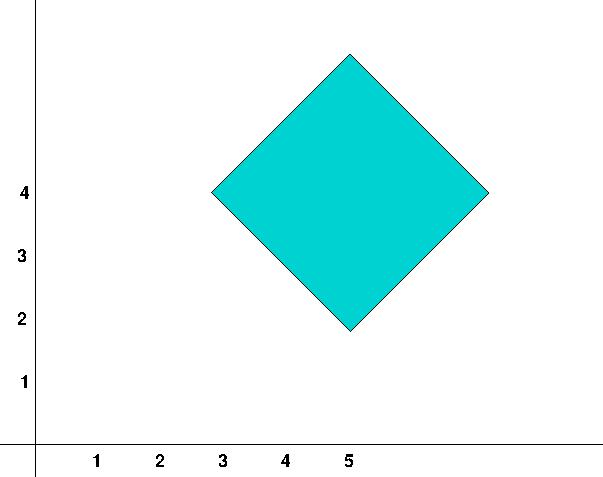
\includegraphics[scale=0.3]{Q3Images/square3.jpg} 
	\centerline{\label{fig3b} \small (3b) Quadrado de lado 3}
\end{minipage}
\end{figure}

%
%
%
\item[{\bf Q4.}] \textbf{Apenas para os alunos de pós-graduação} 
\begin{itemize}
\item Leia o artigo do Torre e do Poggio
  \url{ftp://publications.ai.mit.edu/ai-publications/pdf/AIM-768.pdf}
  e faça um resumo de acordo com as indicações que deixei no
  paca (artigos sobre como fazer um resumo). 
\item O que é um problema mal-posto?
\item O que é regularização? 
\item Qual a importância do teorema apresentado no artigo?
\item O que são filtros de banda limitada? Qual a sua importância no
  artigo?
\item Quais são os métodos de encontrar borda apresentados no artigo?
\end{itemize}
\end{itemize}

\printbibliography
\end{document}
